\documentclass[12pt,fleqn]{article}\usepackage{../common}
\begin{document}
Entegralleri Nasil Dusunelim

Calculus kitaplarinda entegralleri anlatmak icin cogu zaman ``toplam''
kavrami on plana cikarilir, mesela entegralin alttaki resimde $f(x)$
fonksiyonunun altinda kalan ufak ufak dikdortgenlerinin alanlarinin
``toplami'' oldugundan bahsedilir.

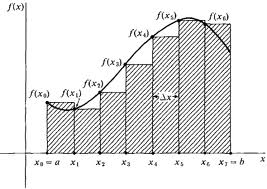
\includegraphics[height=4cm]{area.png}

Fakat bu tur bir anlatim bazen karisikliga yol acabiliyor. Daha iyi bir
anlatim entegralin ``degisen degerlerin carpimi'' oldugudur. Alttaki
resimdeki dikdortgeni dusunelim, 

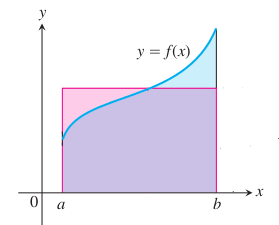
\includegraphics[height=4cm]{box.png}

ve diyelim ki bir dikdortgen, entegralin hesapladigi alani yaklasiksal
olarak temsil ediyor. Dikdortgen alani nasil hesaplanir? Iki kenarinin
carpilmasiyla! Entegral de aslinda boyle bir hesaptir, sadece kenarlardan
biri sabit degildir, ve surekli degismektedir. Bu tur bir anlayis birimleri
sonuca dahil etmek gerektiginde ise yarar, mesela yatay eksen zaman $t$
ise, ve dikey eksen hiz $v(t)$ ise, katedilen mesafe, $v(t)$ nasil bir
sekilde verilmis olursa olsun,

\[ Mesafe = \int v(t)dt \]

formuluyle hesaplanacaktir. Eger hiz ve zaman sabit olsalar, mesela 5 ile 4
gibi, o zaman hesap son derece basit olacakti, 3 x 4 = 12 ile sonucu
bulacaktik. 

Tabii ki carpmak ile toplamak arasinda yakin baglantilar var, mesela 3 x
4'u su sekilde resmedelim

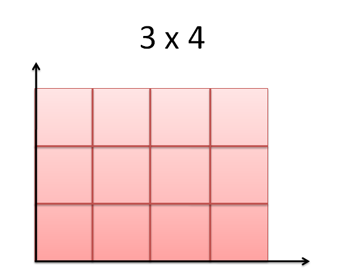
\includegraphics[height=4cm]{grid-multiplication.png}

Burada, evet, 3 degerini dort kere birbiriyle topluyoruz, 3 + 3 + 3 + 3 =
12 ve bu durum 3 x 4 ile ayni sonucu veriyor. Fakat 3'lerin toplami, egri
altindaki alan zihniyetini daha ilerletmeden azicik farkli bir durumu
dusunelim. 

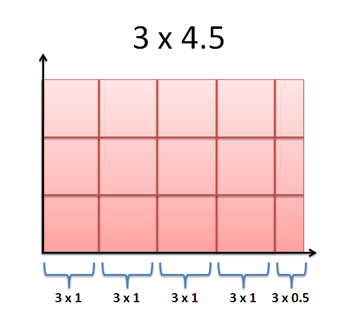
\includegraphics[height=4cm]{piecewise-multiplication.png}

Bu durumda dikey eksendeki kolonlara bir ek yaptik, ama bu ekin genisligi
tam bir kolon degil, yarim bir kolon. Bu durumda alan hesabini sadece dikey
kolonlarin toplanmasi olarak yapsakdik 3'u bes kere toplamamiz gerekirdi,
ve 15 elde ederdik, yanlis bir hesap yapmis olurduk.

Toplamin dogru olmasi icin yatay eksenin genisliginin hesaba katilmasi
gerekir, 3*1 + 3*1 + 3*1 + 3*1 + 3*0.5 = 13.5. Ya da tum genisligi tum
yukseklik ile carpariz 3 * 4.5 = 13.5. 

Peki ilk ornege donersek, madem carpimlardan bahsediyoruz, diyelim ki
$v(t)
= 2t$ o zaman $t
\cdot 2t$ diyemez miyiz? Bu da olmaz, cunku $t\cdot 2t = 2t^2$ 
bize sadece tek bir $t$ anindaki bir hesabi veriyor. Biz verilen bir 
baslangic ve bitis noktalari arasindaki ``tum $t$'ler uzerindeki'' 
katedilen mesafeyle ilgileniyoruz.  

Yani entegral denince aklimiza carpim gelsin, $x,y$ eksenleri baglaminda,
$y$ eksenindeki $f(x)$'i $x$'i carpiyoruz, bu carpim $x$ icin entegrale
$dx$ olarak yansiyor, $f(x)$ ise entegre edilen fonksiyon haline geliyor. 

Birimleri hesaba katarsak anlatilanlar biraz daha anlamlanir belki. Eger
hiz km / saat ise, zaman saat ise, sadece hizlarin toplami mesafe birimini
km / saat yapar, bu yanlis olur. Ama carpim olarak dusunursek km / saat *
saat = km sonucunu verir ki bu mesafenin birimidir. 

Kaynaklar

http://betterexplained.com/articles/a-calculus-analogy-integrals-as-multiplication/

\end{document}
